\documentclass{beamer}

\usepackage[icelandic]{babel}
\usepackage[T1]{fontenc}
\usepackage{graphicx}
\usepackage{fontspec}

\usepackage[rounded]{syntax}
\usepackage{hyperref} 

\hypersetup{pdfencoding=auto}
\setmainfont{Arial} 
\usetheme{hipresentation}
\graphicspath{{./figs/}{../poster/figs/}}

\newenvironment{repnull}[0]{%
\begin{stack}
\\
\begin{rep}
}{%
\end{rep}
\end{stack}
}
\newenvironment{syntaxenv}[1]{%
\par\noindent\begin{minipage}{\linewidth}\vspace{0.5em}\begin{quote}\noindent%
\hspace*{-2em}\synt{#1}:\hfill\par%
\noindent%
\begin{minipage}{\linewidth}\begin{syntdiag}%
}{%
\end{syntdiag}\end{minipage}\end{quote}\end{minipage}%
}

\title{Nútímaleg vefkennsla í notkun gagnasafna með opnum hugbúnaði} 
\author{Eiríkur Ernir Þorsteinsson}
\institute{Háskóli Íslands}
\date{2017}

\begin{document}
{
    \usebackgroundtemplate{
\includegraphics[width=\paperwidth, height=\textheight,keepaspectratio=true]{HI-hattur-verknatt-vector}}
    \frame{\titlepage}
}

\section{Forsaga}

\begin{frame}{Uppruni verkefnisins}
    \begin{columns}
        \column{0.6\textwidth}
        \begin{itemize}
            \item Verkefnið rekur uppruna sinn til kennslubókar sem skrifuð var sumarið 2014
            \begin{itemize}
                \item Notuð í Tækniskólanum
                \item Opin, aðgengileg á Github
            \end{itemize}
            \item Bókinni var dreift á .pdf sniði
            \begin{itemize}
                \item En námsfyrirkomulagið var verklegt
                \item Ljóst að vefur hefði getað þjónað nemendum betur
                \item ``Langt bil'' á milli textans og æfinga
            \end{itemize}
        \end{itemize}
        \column{0.4\textwidth}
        \begin{figure}
            \caption{Forveri verkefnisins}
            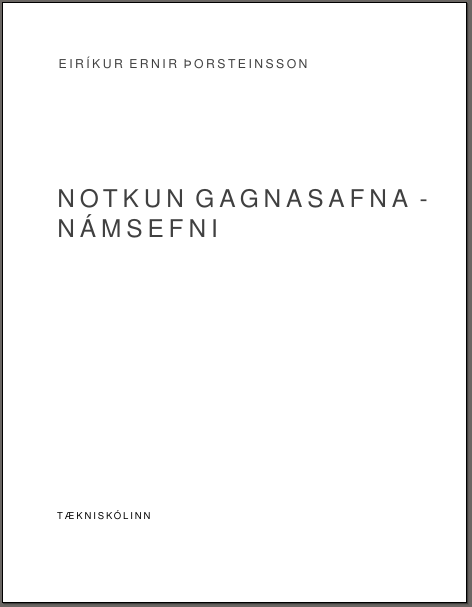
\includegraphics[width=\textwidth]{notkun-gagnasafna}
        \end{figure}
    \end{columns}
\end{frame}

\begin{frame}{Eiginleikar vefsins}
    \begin{itemize}
        \item Fjölmörg önnur kennslukerfi eru til, ekkert hentaði fullkomlega
        \begin{itemize}
            \item Innan háskóla: SQL-Tutor, AsseSQL, LEARN-SQL, \ldots
            \item Utan háskóla: Khan Academy, Coursera, SQLZoo, \ldots
        \end{itemize}
        \item Nokkur atriði eru aðgreinandi fyrir vefinn, en hann\ldots
        \begin{itemize}
            \item styður íslensku
            \item leyfir nemendadrifna, ólínulega framvindu í gegnum efnisatriði
            \item býður upp á verklegar æfingar samþættar við lesefni
        \end{itemize}
    \end{itemize}
\end{frame}

\section{Einkennandi atriði}

\begin{frame}{Vefurinn sem bók, ólínuleg framvinda}
    \begin{columns}
        \column{0.6\textwidth}
        \begin{itemize}
            \item Í hefðbundnari bókum byggist sjálfgefin lestrarröð á efnislegri uppbyggingu
            \begin{itemize}
                \item Röðin er línuleg
                \item Rafbækur engin undantekning
            \end{itemize}
            \item Vefurinn styður \emph{ólínulega framvindu}
            \begin{itemize}
                \item Nemandanum leyft að ráða för
            \end{itemize}
            \item Efnistexta skipt niður í greinar
            \begin{itemize}
                \item Efnishöfundur skilgreinir tengingar á milli greina
                \item Tengingarnar notaðar til að ráðleggja nemendum
            \end{itemize}
        \end{itemize}
        \column{0.4\textwidth}
        \begin{figure}
            \caption{Venslaðar greinar}
            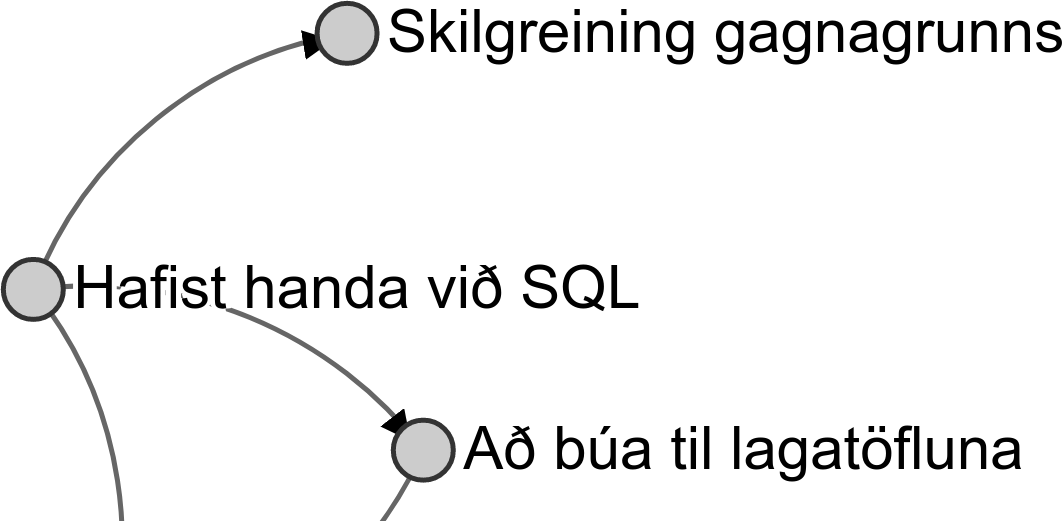
\includegraphics[width=\textwidth]{relational-sections}
        \end{figure}
    \end{columns}
\end{frame}

\begin{frame}{Samþætting texta og æfinga}
    \begin{columns}
        \column{0.6\textwidth}
        \begin{itemize}
            \item Algengt er að kennslukerfi séu fyrst og fremst æfingakerfi
            \begin{itemize}
                \item Texti eingöngu til útskýringar á hverri æfingu fyrir sig
                \item Stundum er texta skipt út fyrir myndbönd
            \end{itemize}
            \item Kennsluvefurinn styður samþættingu efnistextans og æfinganna
            \begin{itemize}
                \item Beinar tengingar, samræmt útlit
            \end{itemize}
        \end{itemize}
        \column{0.4\textwidth}
        \begin{figure}
            \caption{Hægt er að tengja hverja grein við aðrar greinar og/eða æfingar}
            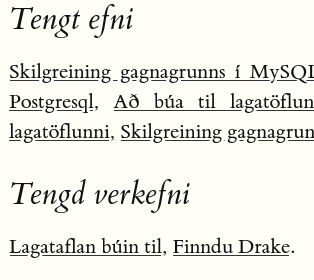
\includegraphics[width=\linewidth]{suggestions}
        \end{figure}
    \end{columns}
\end{frame}

\begin{frame}{Opin hugmyndafræði}
    \begin{columns}
        \column{0.6\textwidth}
        \begin{itemize}
            \item Kennsluvefurinn er opinn á þrjá vegu
            \begin{itemize}
                \item Allur grunnkóði vefsins er opinn
                \item Tæknilausnir frá 3. aðila eru opnar
                \item Efnistexti er gefinn út undir opnu leyfi
            \end{itemize}
            \item Upprunalegur hvati: erfitt er að nálgast grunnkóða eldri kennslukerfa
        \end{itemize}
        \column{0.4\textwidth}
        \begin{figure}
            \caption{Allt textaefni vefsins er aðgengilegt undir Creative Commons leyfi.}
            
\includegraphics[width=\linewidth]{cc-by-nc-sa}
        \end{figure}
    \end{columns}
\end{frame}

\section{Útfærsla}

\begin{frame}{Útfærsla vefsins}
    \begin{columns}
        \column{0.6\textwidth}
        \begin{itemize}
            \item Vefurinn er skrifaður í Python með notkun Django
            \item Önnur tækni sem kemur við sögu:
            \begin{itemize}
                \item SQLite
                \item Tufte CSS
                \item D3.js
                \item Python Markdown
            \end{itemize}
        \end{itemize}
        \column{0.4\textwidth}
        \begin{figure}
            \caption{Vörumerki Python og Django}
            
\includegraphics[width=0.6\linewidth]{python-logo}
            \vspace{1cm}
            
\includegraphics[width=0.8\linewidth]{django-logo}
        \end{figure}
    \end{columns}
\end{frame}

\begin{frame}{Sérhæfðar Markdown viðbætur}
Textainnsetning á vefnum er á Markdown-sniði. Til að styðja við efnisinnsetningu voru fjórar viðbætur við Markdown-túlk skrifaðar sérstaklega fyrir kennsluvefinn.
\begin{center}
    \begin{minipage}{0.9\textwidth}
        \begin{figure}
            \caption{Mállýsingar tveggja viðbóta sem skrifaðar voru fyrir kennsluvefinn}
            \label{fig:markdown-internal-link}
            \begin{syntaxenv}{markdown-internal-link}
                `[' `[' <identifier>
                \begin{stack}
                    `|' <label>\\
                \end{stack}
                `]' `]'
            \end{syntaxenv}
            \begin{syntaxenv}{markdown-footnote}
                `[' `\textasciicircum' <note-identifier> `]' `[' <contents> `]'
            \end{syntaxenv}
        \end{figure}
    \end{minipage}
\end{center}
\end{frame}

\begin{frame}{Markviss textaframsetning}
    \begin{itemize}
        \item Þar sem kennsluvefurinn skal gegna hlutverki kennslubókar er textaframsetning mikilvæg
        \item Hönnun einkennist af notkun css-safnsins Tufte CSS 
        \begin{itemize}
            \item Mikil notkun spássíugreina
            \item Samþjöppun texta og mynda
            \item Markviss notkun lita og leturgerða
        \end{itemize}
    \end{itemize}
    \begin{figure}
        \caption{Texti og mynd birt samhliða}
        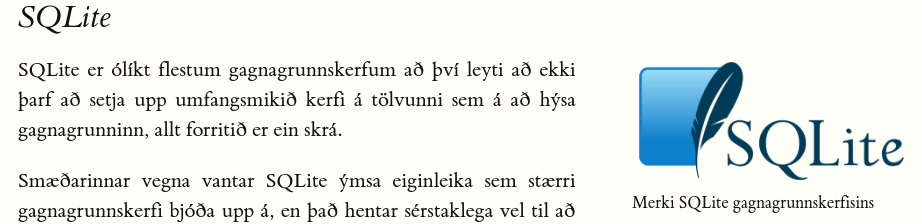
\includegraphics[width=\linewidth]{sqlite}
    \end{figure}
\end{frame}

\begin{frame}{Greining nemendafyrirspurna}
    \begin{columns}
    \column{0.6\linewidth}
        \begin{itemize}
        \item Greining á SQL-fyrirspurnum er ekki leyst vandamál
        \item Kennsluvefurinn fer tvær einfaldar leiðir
        \begin{itemize}
            \item Samanburður á niðurstöðumengjum er notaður þegar honum verður komið við
            \item Þegar slíkt er ekki mögulegt er einfaldur textasamanburður notaður
        \end{itemize}
    \end{itemize}
    \column{0.4\linewidth}
    \begin{figure}
        \caption{Sjálfgefið flæði þegar fyrirspurn er metin}
        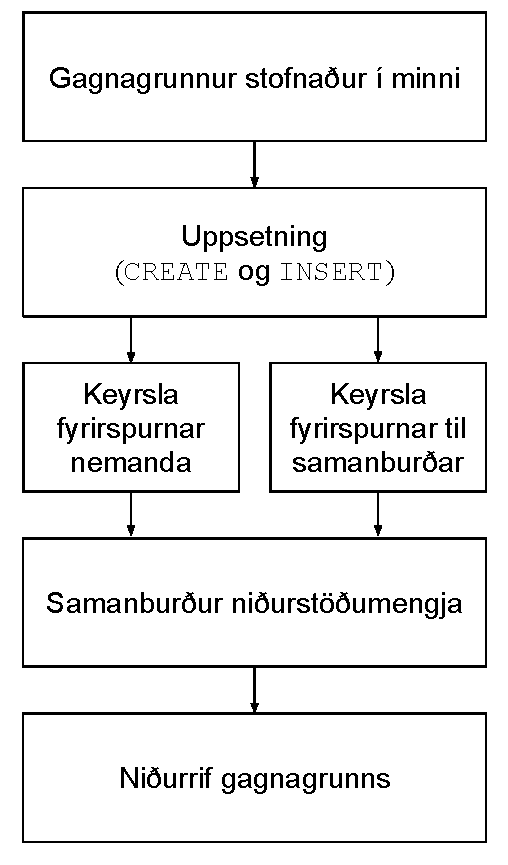
\includegraphics[width=0.8\linewidth]{keyrsla-fyrirspurnar-lodrett}
    \end{figure}
    \end{columns}
\end{frame}

\section{Framtíðarsýn}

\begin{frame}{Næstu skref}
    \begin{itemize}
        \item Vefurinn er tilbúinn til tilraunanotkunar
        \item En rannsóknarvinna liggur fyrir
        \begin{itemize}
            \item Er þessi gerð efnisframsetningar vænleg til árangurs?
            \item Er pláss fyrir opið kennsluefni í íslenska menntakerfinu?
        \end{itemize}
        \item Tæknilegar betrumbætur í augsýn
        \begin{itemize}
            \item Greining fyrirspurnanna er frumstæð
            \item Efnisinnsetningu má auðvelda enn frekar
            \item Bæta skrásetningu og framsetningu á gögnum sem safnast
            \item Hönnun og myndanotkun þarfnast yfirferðar
        \end{itemize}
    \end{itemize}
\end{frame}

\begin{frame}{Sækið kóðann!}
    \begin{center}
        
\includegraphics[height=0.65\textheight]{qr-code}

        \url{https://github.com/Ernir/sql-web}
    \end{center}
\end{frame}

\end{document}